\documentclass{mcmthesis}
\mcmsetup{CTeX = false,   % 使用 CTeX 套装时,设置为 true
        tcn = 78435, problem = E,
        sheet = true, titleinsheet = true, keywordsinsheet = true,
        titlepage = false, abstract = true}
\usepackage{palatino}
\usepackage{float}
\usepackage{etoc}
\usepackage{array}
\newcolumntype{I}{!{\vrule width 3pt}}
\newlength\savedwidth
\newcommand\whline{\noalign{\global\savedwidth\arrayrulewidth
                            \global\arrayrulewidth 1.2pt}%
                   \hline
                   \noalign{\global\arrayrulewidth\savedwidth}}
\newlength\savewidth
\newcommand\shline{\noalign{\global\savewidth\arrayrulewidth
                            \global\arrayrulewidth 1.2pt}%
                   \hline
                   \noalign{\global\arrayrulewidth\savewidth}}
\title{How does climate change influence regional instability?}
\author{}
\date{}
\begin{document}
\begin{abstract}
In the present airport construction, the reliability and efficiency of security inspection are of vital significance, while the occurrence of congestion in checkpoints is undeniably frequent. This report aims to analyze the current process of airport security checkpoints and propose rational modifications.

Firstly, we do the parameter analysis and process division based on the current situation and data. We assume that the flow of passengers obeys \textbf{PoissonDistribution}, and that the checking time obeys \textbf{Exponential Distribution}. According to the data given, we estimate related parameters using \textbf{Moment Estimation}, and obtain the quantitative model. Meanwhile, we perform the integral analysis of the system and figure out the relationship between the maximal flow of passengers and the proportion of ID-Check entrance number to screening lane number. After the simulation, we conclude that the bottleneck appears owing to screening lanes.

Secondly, we propose two modifications to our model. According to the time consumed in different areas, we figure out the ideal proportion of the number of entrances and lanes so as to reach the highest throughput. Applying the M/M/S model in \textbf{Queuing Theory}, we obtain several \textbf{dynamic optimization} functions based on the principle of minimizing the fluctuation of the average waiting time. Considering both mentalities of passengers and construction costs of airports, we attain the final optimization. 

Thirdly, we do \textbf{sensitivity analysis} of the modified model. In previous analysis, we assume that passengers all obey rules and act normally, but due to discrepancies of cultural environment, passengers tend to behavior diversely, which could impact our model. Therefore, we mainly analyze three types of passengers and impacts of their behaviors on our model. Passengers who are queue-jumpers may cause disputes leading to the paralysis of specific entrances, and those who dress special may prolong the screening time. Furthermore, ones who hold obscure perception of contraband may be more prone to get additional screening.

Finally, we propose policy and recommendations for security managers based on our optimal model. For instance, rearrange the number of entrances or lanes according to the current throughput, establish a baggage buffer at the end of X-ray belts, and promote Pre-Check.



\begin{keywords}
Parameter Estimation; Queuing Theory; Dynamic Optimization; Maximal Throughput; Airport Security; Cultural Diversity
\end{keywords}
\end{abstract}
\maketitle

\newpage
\begin{center}
	\tableofcontents
	\setcounter{page}{0}
	\thispagestyle{empty}
\end{center}
\newpage

\section{Introduction}

A \textbf{fragile state} is a low-income country or a sovereign state that is characterized by weak state capacity and/or weak state legitimacy[1]. It increases the vulnerability of citizens towards a range of shocks, including economic fluctuation, political upheaval, and so forth. 

Particularly, \textbf{climate shock} such as unpredictable natural disasters, extreme weather, decreasing cultivated land and changing ranges of plants and animals may dramatically aggravate fragile states and may further leads to regional violent conflicts when social fragmentation and weak governance exist as well. Therefore, it is of vital significance to research on how climate change will affect the instability or fragility of a state and how human intervention can mitigate such negative impact.

In this paper, we mainly focus on analyzing the influence of climate change on regional instability and fragility. More specifically, we pay attention to the following issues:
\begin{itemize}
	\item Develop a model that determines the fragility of a country and identify when a state is fragile, vulnerable, or stable. Simultaneously, the model will measure the impact of climate change and analyze direct and indirect means by which climate change increases the fragility.
	\item Select A, one of the top 10 most fragile states as determined by the Fragile State Index (http://fundforpeace.org/fsi/data/) and use the model to analyze how climate change has increased the fragility of it and show in what way(s) A may be less fragile without these effects.
	\item Apply the model on B to measure its fragility, and determine in what way and when climate change may increase the fragility of the state. Identify any definitive indicators. Define a tipping point and predict when B may reach it.
	\item Use the model to show which state driven interventions could alleviate the risk of climate change and prevent a country from becoming a fragile state. Explain the effect of human intervention and predict the total cost of intervention for this country.
	\item Analyze whether the model will correctly work on smaller “states” (such as cities) or larger “states” (such as continents) and modify the models accordingly.
	\item Assess strengths and weaknesses of the model.
\end{itemize}

In the following chapters, we will demonstrate and illustrate our model in details, as well as evaluating the model in all directions.

\section{Assumption}

\begin{itemize}
\item Assume that climate change is random and cannot be controlled by human.

\item Assume that the variation of economy, society and policy factors in a country is only dependent on current country status if there is no climate change.

\item Assume that there is no sudden revolution in the country analyzed.

\item Assume the time delay between climate change and national response is short enough.

\item Assume that all countries have the same evaluation function and prediction function.

\end{itemize}

\section{A model for current process}
In this section, we draw a relationship schema of several vital factors to show the direct influences between them. Take economic policy as an example, it has a strong direct effect on GDP under most circumstances. And in the schema, we can also see the indirect influence since all the boxes are connected by arrow lines. After that, an evaluation function can be determined by weighting the factors’ contribution to fragility. Even more, we can also gain a recursion function to predict the country’s fragility in a few years. Using these functions to evaluate current status of some typical countries, an evaluation standard then be settled.
\subsection{Model establishing}
Based on the schema, we focus on several factors that might have the most impact on a country's fragility. Policies issued by government, military activities, social problems and economic crisis are four major factors effecting fragility. These factors also have interconnections, which makes this model more realistic and manageable.

\begin{figure}[h]
	\small
	\centering
	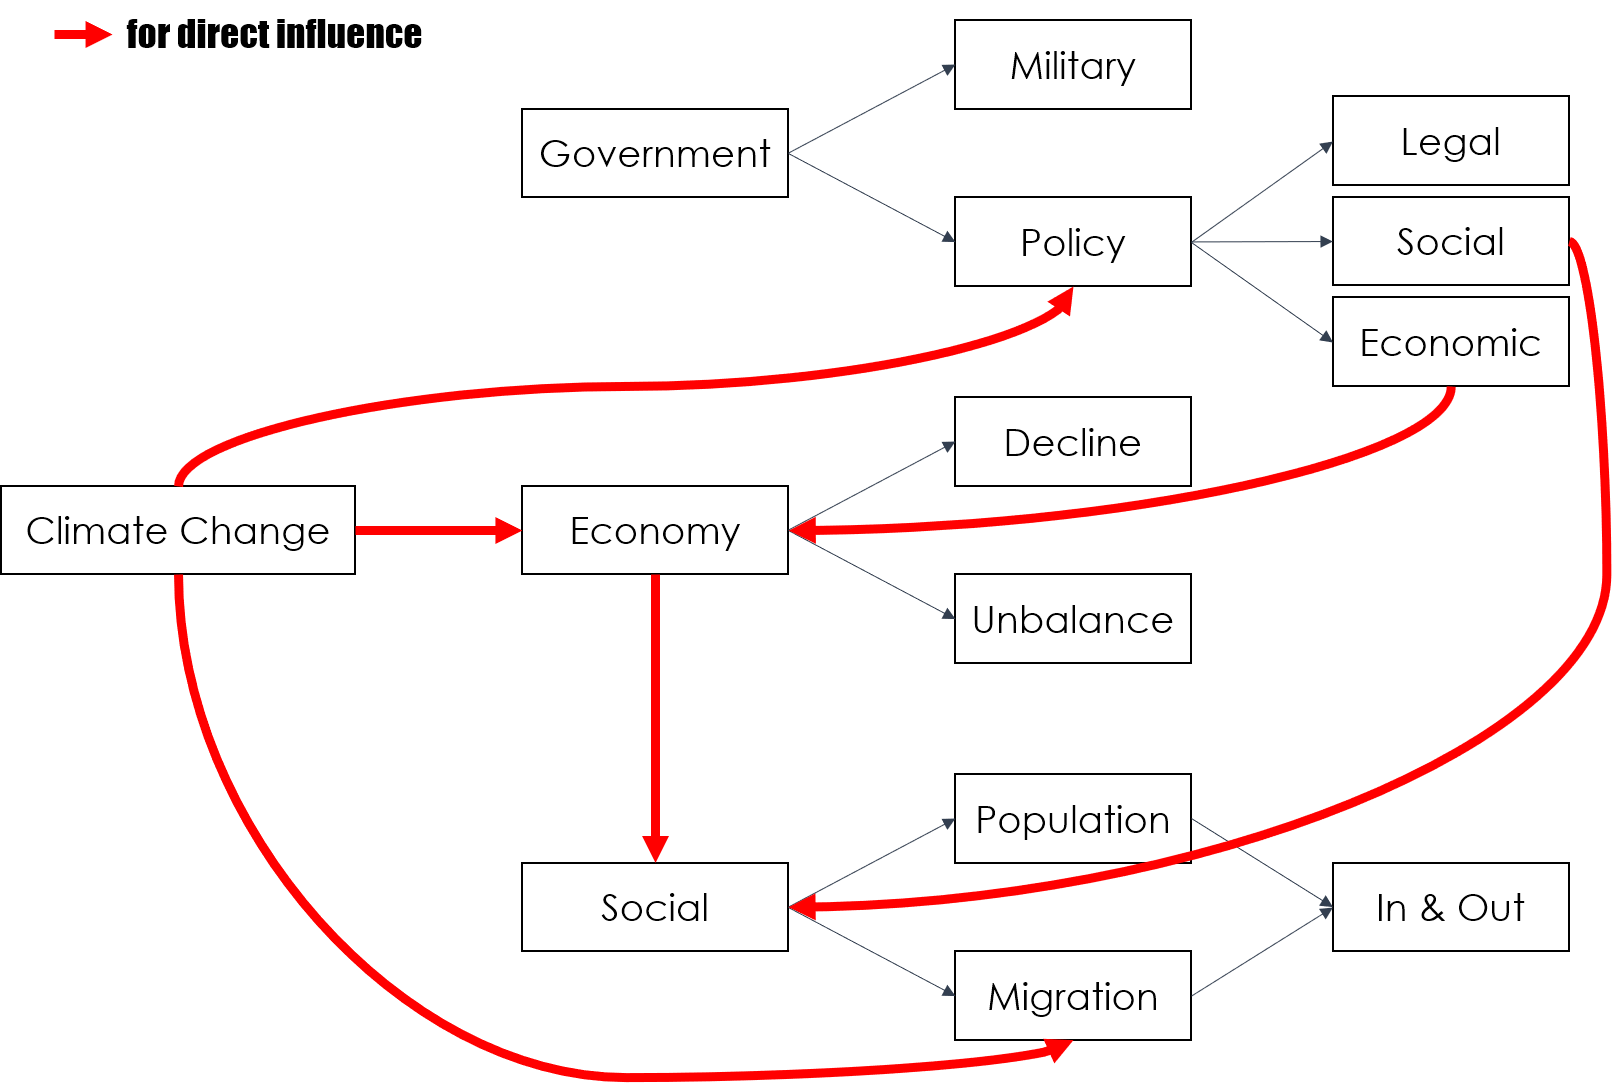
\includegraphics[width=15cm]{figure2.png}
	\caption{Stage-structured model of current process} \label{fig:Stage-structured model of current process}
\end{figure}

\noindent Additionally, the quantities involved in the function are shown in \textbf{Table 1} and \textbf{Table 2}. We list subscripts and primary notations apart.\\

\begin{table}[htbp]
	\renewcommand\arraystretch{1.5}
	\footnotesize
	\centering
	\begin{tabular}{m{3cm}<{\centering}|m{10cm}<{\centering}}
		\whline
		\textbf{Subscript}&\textbf{Definition}\\
		\whline 
		$N$&$N_{th}$ year\\ 
		\shline
	\end{tabular}
	\caption{Definition of Subscripts in the model}\label{tab:Definition of Subscripts in the model}
\end{table}
\begin{table}[htbp]
	\renewcommand\arraystretch{1.5}
	\footnotesize
	\centering
	\begin{tabular}{m{3cm}<{\centering}|m{10cm}<{\centering}}
		\whline
		\textbf{Notation}&\textbf{Definition}\\
		\whline 
		$F$&Degree of Fragility\\
		$C$&Climate factor\\
		$E$&Economic factor\\
		$S$&Social factor\\
		$P$&Policy factor\\ 
		$M$&Military factor\\
		$X$&External Intervention\\
		\shline
	\end{tabular}
	\caption{Definition of notations in the model}\label{tab:Definition of notations in the model}
\end{table}

As assumed, if climate and external intervention remains zero, our major factors should be a \textbf{Markov Model}, which is

$$
\left(
\begin{matrix}
	P_{N+1} \\ M_{N+1} \\ E_{N+1} \\ S_{N+1}
\end{matrix}
\right) 
= 
\left(
\begin{matrix}
k_{11} & k_{12} & k_{13} & k_{14} \\
k_{21} & k_{22} & k_{23} & k_{24} \\
k_{31} & k_{32} & k_{33} & k_{34} \\
k_{41} & k_{42} & k_{43} & k_{44} \\
\end{matrix}
\right) 
\left(
\begin{matrix}
P_N \\ M_N \\ E_N \\ S_N
\end{matrix}
\right) 
$$

\begin{table}[htbp]
	\renewcommand\arraystretch{1.5}
	\footnotesize
	\centering
	\begin{tabular}{m{2.7cm}<{\centering}|m{5cm}<{\centering}|m{5cm}<{\centering}}
		\whline
		\textbf{Hypothesis}&\textbf{$P_N$}&\textbf{$M_N$}\\
		\whline
		\textbf{Short-term insufficient or excessive precipitation}& 2 support, 1 none, 1 opposite &1 support, 2 none, 1 opposite\\
		
		\textbf{Short-term temperature increase or decrease}&1 support, 2 none, 1 opposite&1 support, 1 none, 1 opposite\\
		
		\textbf{Natural disasters}&2 support, 1 opposite&1 none\\
		
		\textbf{Sea level rising}&2 support, 1 none, 1 opposite&1 support, 1 none, 1 opposite\\
		
		\textbf{Energy deficiency}&2 support, 1 opposite&3 none\\
		
		\textbf{Less vegetation}&2 none&1 none\\
		
		\shline
		\textbf{Hypothesis}&\textbf{$E_N$}&\textbf{$S_N$}\\
		\whline
		\textbf{Short-term insufficient or excessive precipitation}& 3 support, 1 some support &2 support, 1 opposite\\

		\textbf{Short-term temperature increase or decrease}&4 support, 1 none, 2 opposite&2 support, 1 none, 1 opposite\\

		\textbf{Natural disasters}&6 support, 1 opposite&6 support, 2 opposite\\

		\textbf{Sea level rising}&3 support, 1 none, 1 opposite&2 none\\

		\textbf{Energy deficiency}&2 support, 1 opposite&2 support, 1 none, 1 opposite\\

		\textbf{Less vegetation}&3 support, 1 none, 1 opposite&2 support, 1 opposite\\
		\shline
	\end{tabular}
	\caption{Influence of climate change}\label{tab:Influence of climate change}
\end{table}

\begin{table}[htbp]
	\renewcommand\arraystretch{1.5}
	\footnotesize
	\centering
	\begin{tabular}{m{2.7cm}<{\centering}|m{5cm}<{\centering}|m{5cm}<{\centering}}
		\whline
		\textbf{Hypothesis}&\textbf{$P_N$}&\textbf{$M_N$}\\
		\whline
		\textbf{$P_N$}&3 support &2 support, 1 none, 2 opposite\\

		\textbf{$M_N$}&2 support, 1 none, 2 opposite&4 support\\

		\textbf{$E_N$}&4 support, 1 none&1 support, 1 opposite\\

		\textbf{$S_N$}&1 support, 1 none&2 support, 1 none, 1 opposite\\
		\shline
		\textbf{Hypothesis}&\textbf{$E_N$}&\textbf{$S_N$}\\
		\whline
		\textbf{$P_N$}& 3 support, 1 none, 1 opposite & 1 support, 1 none\\

		\textbf{$M_N$}&1 support, 2 none&1 support, 1 none\\

		\textbf{$E_N$}&3 support&1 support, 2 none\\

		\textbf{$S_N$}&1 support, 2 none&1 support\\
		\shline
	\end{tabular}
	\caption{Interplay of different factors}\label{tab:Interplay of different factors}
\end{table}

For the ID-check, the basic sketch is shown in \textbf{Figure 3}.
\begin{figure}[h]
\small
\centering
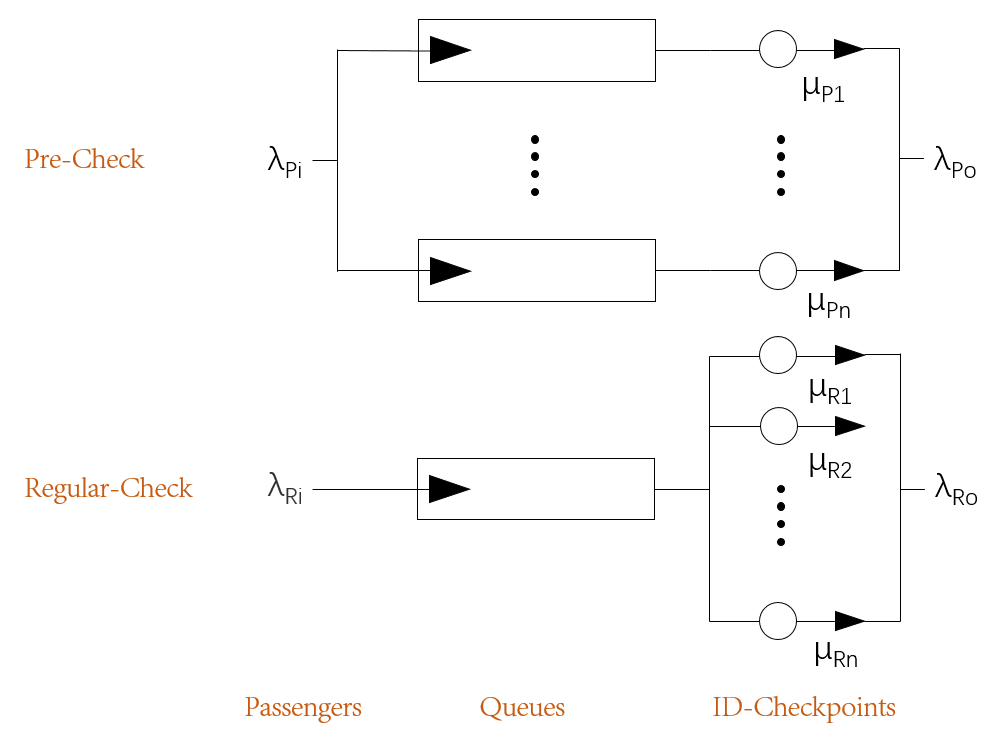
\includegraphics[width=10cm]{figure3.png}
\caption{Basic sketch for ID-check} \label{fig:Basic sketch for ID-check}
\end{figure}\\
For the screening lanes, the basic sketch is shown in \textbf{Figure 4}.

\begin{figure}[h]
\small
\centering
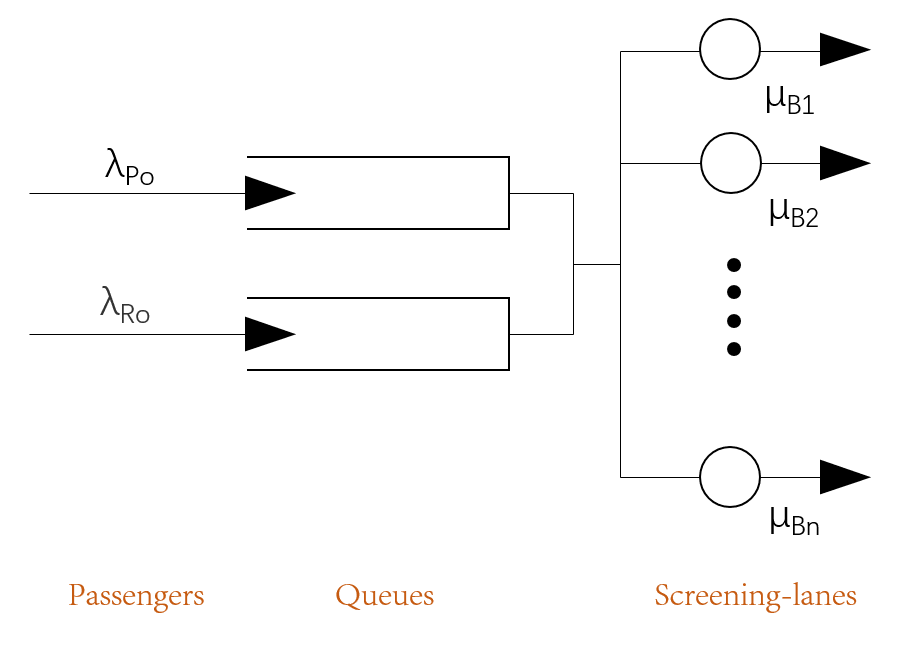
\includegraphics[width=10cm]{figure4.png}
\caption{Basic sketch for screening lanes} \label{fig:Basic sketch for screening lanes}
\end{figure}
In order to build the model clearly and precisely, we have to make some assumptions. Since the data of most airports are inaccessible, we assume the distribution functions of the flow of passengers, of time for ID check and of time for security check as below.
\begin{itemize}
\item The number of arriving passengers per second is subject to Poisson Distribution. For the Pre-Check Entrance and Regular Entrance, we have
$$P(\lambda_{Pi}=k)=\frac{e^{-\lambda_P}(\lambda_P)^k}{k!}$$
$$P(\lambda_{Ri}=k)=\frac{e^{-\lambda_R}(\lambda_R)^k}{k!}$$
\item The time it takes at each ID-Checkpoint per person is subject to exponential distribution
$$F(t)=1-e^{-\mu_At}$$
\item The time it takes to pass Zone B per person is subject to exponential distribution as well
$$F(t)=1-e^{-\mu_Bt}$$
\end{itemize}
\subsection{Estimation for some parameters}
Based on data we have received, we can attain the estimated value for $\lambda_P$, $\lambda_R$, $\mu_A$, and $\mu_B$ ( See details about the data in \textbf{Appendix A}). We use Successive Minus to calculate the average value. For the number of the arriving passengers per second, the average time interval $\overline{\Delta t_P}$ between every 29 persons at the Pre-Checkpoint is 286.6s. Therefore, due to Moment Estimation, $\lambda_P$ is given by
$$\widehat{\lambda_P}=\frac{\overline{n_{Pi}}}{\overline{\Delta t_P}}=0.1012s^{-1}$$
By similar method, we can obtain the estimated values for $\lambda_R$ as well ( $\overline{\Delta t_R}$ is the average time interval between every 23 persons at the regular checkpoint )
$$\widehat{\lambda_R}=\frac{\overline{n_{Ri}}}{\overline{\Delta t_R}}=0.0668s^{-1}$$
Existing data provide two samples of ID-Check process time. By calculating the average time costing for each TSA officer and taking the average of these results again$(\overline{t_A})$, we can acquire the estimated value for $\mu_A$
$$\widehat{\mu_A}=\frac{1}{\overline{t_A}}=0.0877s^{-1}$$
Based on the time costed at Zone B for each passenger, we can get $\mu_B$
$$\widehat{\mu_B}=\frac{1}{\overline{t_B}}=0.0349s^{-1}$$
\subsection{Current process analysis}
As the additional screening is not always happening, we can assume the proportion of this unexpected case to be a certain small constant $\eta$. Since $\eta$ is small, every passenger who gets additional searching will not wait in Zone D, as a result, the change of flow can be approximatively ignored. If given the maximum of passenger flow $f_{max}$, the function to describe exit passengers' number is
\begin{equation}
    f_{o}=
   \begin{cases}
   f_{max}, &\mbox{$f_i \geq f_{max}$}\\
   f_i, &\mbox{$f_i < f_{max}$}
   \end{cases}
\end{equation}
Assume that $t_{Pk}, t_{Rk}, t_{Lk}$ are time through the Pre-Check entrance, regular-check entrance and screening lanes for the kth sample, so we can easily find that 
$$f_{max}=min\{\sum_{k=1}^{N_P}\frac{1}{t_{Pk}}+\sum_{k=1}^{N_R}\frac{1}{t_{Rk}},\sum_{k=1}^{N_L}\frac{1}{t_{Lk}}\}$$
We use the estimated values to calculate the numerical solution, since the situation when $f_i<f_{max}$ is quite simple, we only aim to find the max flow for current process, which is the index of the bottleneck.

The simplified function is
$$f_{o max}= min\{\sum_{k=1}^{N_P}\mu_{Pk}+\sum_{k=1}^{N_R}\mu_{Rk},\sum_{k=1}^{N_L}\mu_{Bk}\}$$
As given, $3N_P=N_R$. And the Pre-Check is not faster than regular check at the ID-Checkpoint, so $U_P=U_R=U_A$.
$$f_{o max}= min\{4N_P\mu_A,N_L\mu_B\}$$
\textbf{Figure 5} shows the relationship between $N_L/N_P$ and $f_{omax}$

\begin{figure}[H]
\small
\centering
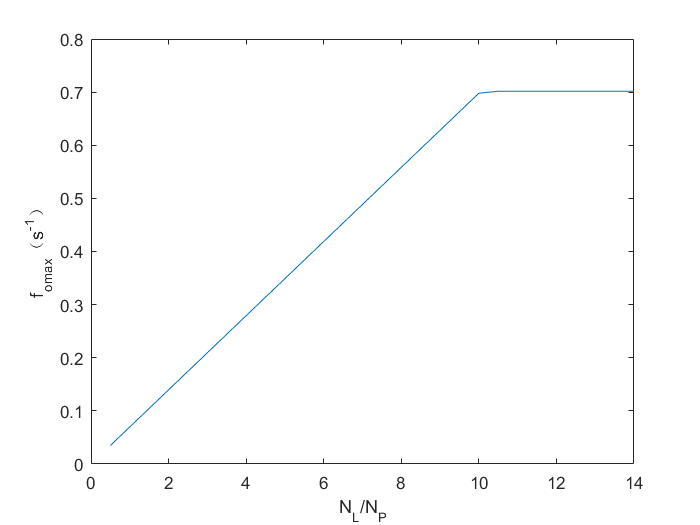
\includegraphics[width=8.5cm]{figure5.png}
\caption{$f_{omax}-N_L/N_P$} \label{fig:$f_{omax}-N_L/N_P$}
\end{figure}
\noindent When $4N_P\mu_A=N_L\mu_B$, which is $N_L\approx10N_P$, $f_{omax}$ reaches its peak. However, if $N_L$ gets larger, there will be unused screening lanes, which lower the efficiency of the whole security system.
\subsection{Assessment and conclusion}
This model is only an estimation of the current operating system at one certain airport, and it has some limitations. First of all, we use moment estimators of passenger flow and passing time to calculate relevant parameters, which suits well mostly under the circumstance that sampling time is long enough and that people' s  arriving possibility is equal all the time. If not, the accuracy of the result can not be completely gauaranteed. Secondly, we did not consider the differences among people. For example, the elder are more likely to act slowlier than youngsters, and we wonder if this difference would cause changes in some parameters. Finally, we did not consider the time saved for those who have bought Pre-Check service, as we did not attain the relevant data. However, it is undeniably an important factor when calculating the passing time of screening.

So, we draw the conclusion that, when all the assumptions are positive, the passenger flow firstly increases as the input flow gets up, then when the ID-Checkpoint or screening check-lanes reach saturation, the flow of departing passengers starts to maintain a stable value. As for the maximum throughput for the current model, we have attained the result that when $N_L/N_P=10$, the flow of departing passengers reaches its peak, which is the bottleneck of the input flow for current model. However, as we can see from the figure given, $N_L/N_P<10$, so the screening check-lanes reach saturation earlier than ID-Checkpoint. As a result, the problem area mainly exists in \textbf{Zone B}.

\section{Modifications for current process}
After analyzing the flow of passengers and existing bottlenecks of the current process of security check, we propose several modifications in order to increase the throughput of passengers and reduce variance in waiting time. Since the calculation of the average waiting time depends on the values of $N_P$, $N_R$, $N_B$ and $N_X$ ( See \textbf{Figure 6}), we first modify the ratio of $N_P$, $N_R$, $N_B$ and $N_X$ so as to maximize the throughput, and on that basis we develop a dynamic optimization fuction to adjust the number of entrances as the flow of passengers entering the checkpoint changes, by which we can minimize variance in waiting time.  
\begin{figure}[h]
\small
\centering
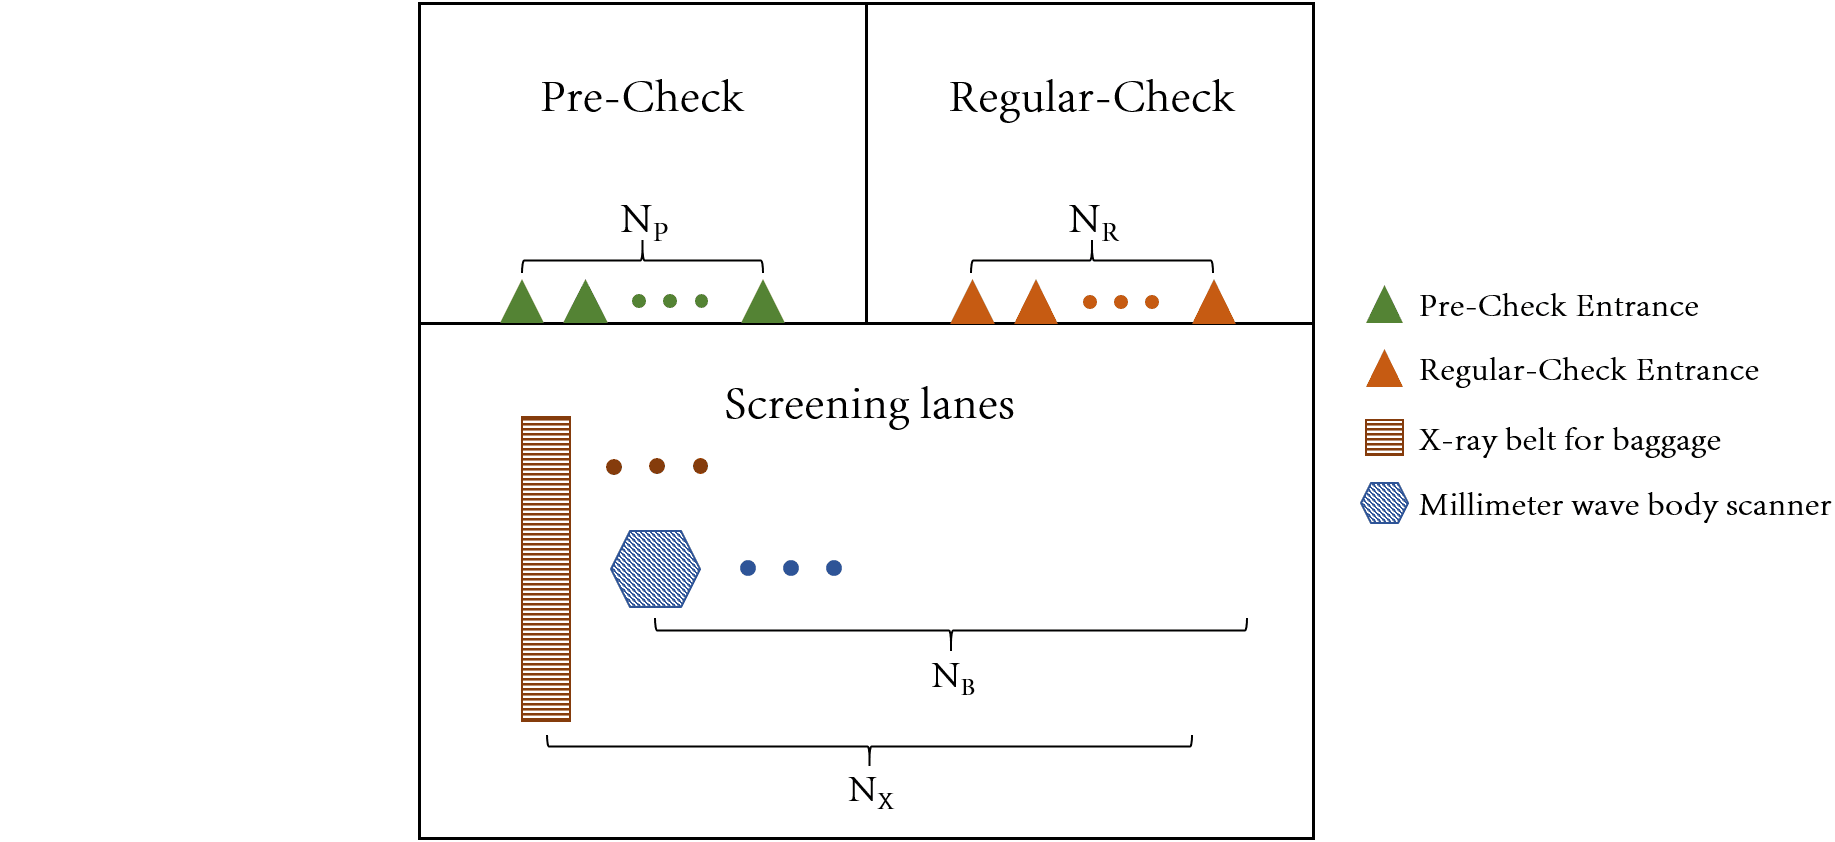
\includegraphics[width=15cm]{figure6.png}
\caption{Skecth of a security checkpoint} \label{fig:Skecth of a security checkpoint}
\end{figure}
\subsection{Modifications for increasing passenger throughput}
We find three small modifications to increase passenger flow when the throughput gets saturated.
\subsubsection{Change ratio of $N_X$ to $N_B$}
We look into the data provided, and find that the time for people's properties getting scanned is much more than the time costed on themselves. So, if we could change $N_X/N_B$ to a more suitable value, the time utilization ratio can be developed. We analyze the data and use Successive Minus to calculate the ratio of average time spent on properties and persons, then we find that
$$t_X:t_B=2.2:1$$
So, when we do not have a large number of screening-lanes, we can set 
$$N_X:N_B=2:1$$
That is to say, when every two people share one millimeter wave body scanner and use two screening belt, the waiting time reach its minimum value and the efficiency of Zone B gets maximum. There is an accurate definition for "waiting" here that one person stops waiting as soon as he(she) puts his(her) baggage on the X-ray belt.
\subsubsection{Change ratio of $N_P$ to $N_R$}
We have calculated the ratio of people choosing Pre-Check to people choosing Regular-Check in our basic model according to the data.
$$\lambda_P:\lambda_R=3:2$$
Generally, we can set the ratio to
$$N_P:N_R=3:2$$
\subsubsection{Change the ratio of $(N_P+N_R)$ to $N_X$}
The modification above applied, the average time for passengers passing the screening-lanes is shortened, and the average flow for each lane is enlarged
$$\widehat{\mu_B}=\frac{1}{\overline{t_B}'}=0.0714s^{-1}$$
$\mu_A$ is still the same value. Thus, due to the stability equation
$$(N_P+N_R)\mu_A=N_X\mu_B$$
We can find when
$$N_X=1.2(N_P+N_R)$$
the whole system is stable and there will be no congestion inside the security checkpoint.
The further modifications are all based on these three basic principles.
\subsection{Modifications for reducing time variance}
In this section, we apply the Queuing Theory Model to simulate the process of security check. According to the Queuing Theory Model, we can obtain a relationship between $W_q$ (average waiting time for every passenger) and $s$ (the number of entrances). In order to minimize the variance of $W_q$, the airport should adjust $s$ based on various flow of passengers entering the checkpoint, which is related to $\lambda$.

According to the assumptions we have already proposed, the number of arriving passengers per unit time obey Poisson Distribution $\pi(\lambda)$, and time passing through the ID-check or screening area obey Exponential Distribution $E(\mu)$. Define $\rho=\frac{\lambda}{s\mu}$. From the Queuing Theory Model, we can obtain the following results:

\begin{itemize}
\item When the number of entrances is $s$, the probability $P_n(s)$ when there are $n$ passengers in the system  is
\begin{equation}
    P_n(s)=
   \begin{cases}
   \frac{(s\rho)^n}{n!}P_0(s), &\mbox{$n=1,2,\ldots,s$}\\
   \frac{s^s\rho^n}{s!}P_0(s)=\rho^{n-s}P_s(s), &\mbox{$n=s+1,s+2,\ldots$}
   \end{cases}
\end{equation}
$$P_0(s)=[\sum_{n=0}^{s-1}\frac{(s\rho)^n}{n!}+\frac{(s\rho)^s}{s!}(\frac{1}{1-\rho})]^{-1}$$
\item The average number of passengers waiting in queues $L_q$ is
$$L_q=\sum_{n=s+1}^{\infty}(n-s)P_n(s)=\frac{(s\rho)^s\rho}{s!(1-\rho)^2}P_0(s)$$
\item The average number of passengers in the checkpoint $L_s$ is 
$$L_S=L_q+s\rho$$
\item The average time waiting in queues $W_q$ is
$$W_q=\frac{L_q}{\lambda}$$
\item The average time spending in the checkpoint $W_s$ is
$$W_s=\frac{L_s}{\lambda}$$
\end{itemize}

More specifically, since in the previous modifiations we rearranged the proportianal relationship between $N_P$ and $N_R$ so as to make sure the passengers uniformly entering every entrances. Therefore, we consider the whole checkpoint as a M/M/S system, where $s$ is the sum of $N_P$ and $N_R$, and $\lambda$ is the number of passengers  arriving at every entrance per unit time. Furthermore, since the total servce time is the sum of time in Zone A and Zone B, $\mu$ can be attained as follows.
$$\mu=\frac{1}{\frac{1}{\mu_A}+\frac{1}{\mu_B}}=0.0433s^{-1}$$
Then, we use Matlab to simulate our model. Firstly, we assign different values to $s$ from 2 to 15 and calculate the corresponding $\lambda$ on condition that $W_q$ keeps constant ($25s$). Results are shown in \textbf{Table 3}.

\begin{table}[htbp]
\centering
\begin{tabular}{m{4cm}<{\centering}m{4cm}<{\centering}}
\toprule
\textbf{$s$}&\textbf{$\lambda\ (s^{-1})$}\\
\midrule
2&0.0866\\

3&0.1299\\

4&0.1732\\

5&0.2156\\

6&0.2598\\

7&0.3031\\

8&0.3464\\

9&0.3897\\

10&0.4330\\ 

11&0.4763\\ 

12&0.5196\\

13&0.5629\\

14&0.6062\\
 
15&0.6495\\
\bottomrule
\end{tabular}
\caption{$s-\lambda$}\label{tab:Data}
\end{table}
From the data above, it can be discovered that $s$ and $\lambda$ are directly propotional. Therefore, assuming that $s$ and $\lambda$ are continuous, we can figure out the fuctional relationship between $\lambda$ and $s$:
$$s=\frac{\lambda}{0.0433}$$
We notice that $\mu=0.0433s^{-1}$, so we can draw the conclution that
$$s=\frac{\lambda}{\mu}$$
Then, we apply different approaches to round $s$ to appropriate integers. See \textbf{Figure 7}.


Moreover, we draw the fitting figure between $W_q$ and $\lambda$ in \textbf{Figure 8} in order to assess different  approaches. In \textbf{Figure 8}, (1) and (2) will lead to long waiting time under specific conditions, which is due to the unstable state of the system. Such unstability is the result of $\rho=\frac{\lambda}{s\mu}>1$. As for (3) and (4), such unstability can be avoided, but (3) brings higher cost. Thus, we apply the approach in (4) to round $s$. 
\begin{figure}[H]
\small
\centering
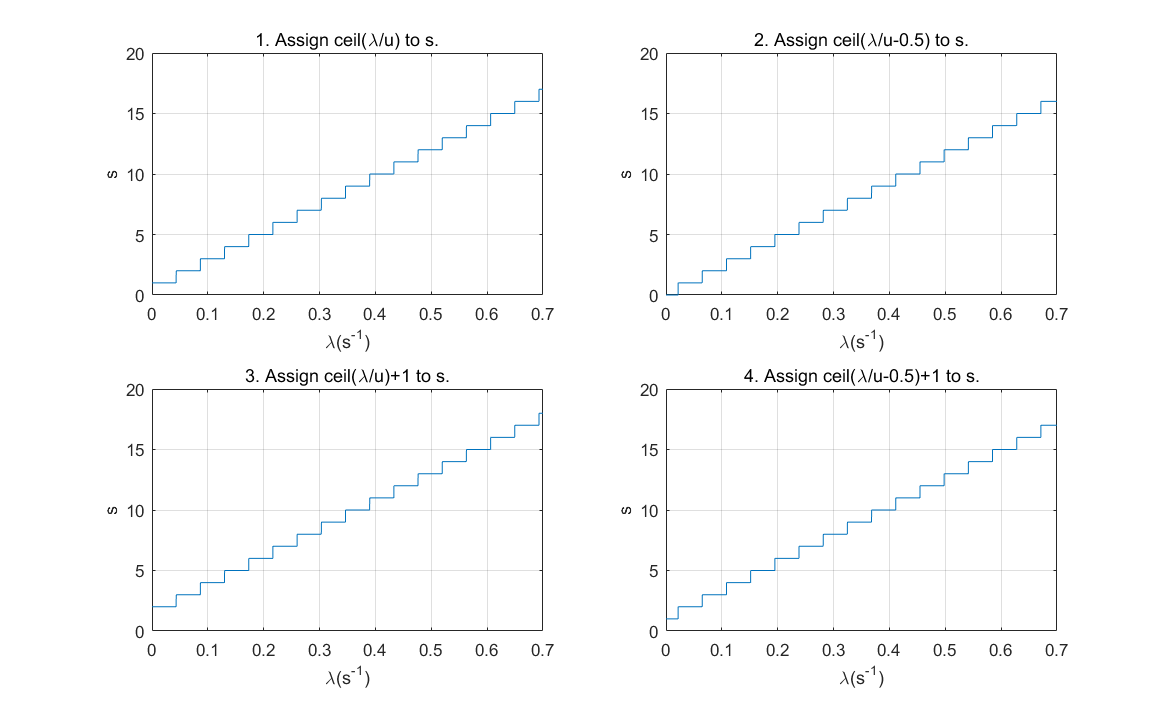
\includegraphics[width=14.5cm]{figure7.png}
\caption{$s-\lambda$ of different approaches} \label{fig:7}
\end{figure} 

In conclution, as $\lambda$ changes, we set $s$ as $s=\lceil\frac{\lambda}{\mu}-0.5\rceil+1$, which means when the flow of passengers entering the checkpoint increase, the airport need to increase the number of entrances according to the relationship above. By this method, we can reduce variance in waiting time by $\Delta W_q \leq \pm19.4s$.
\begin{figure}[H]
\small
\centering
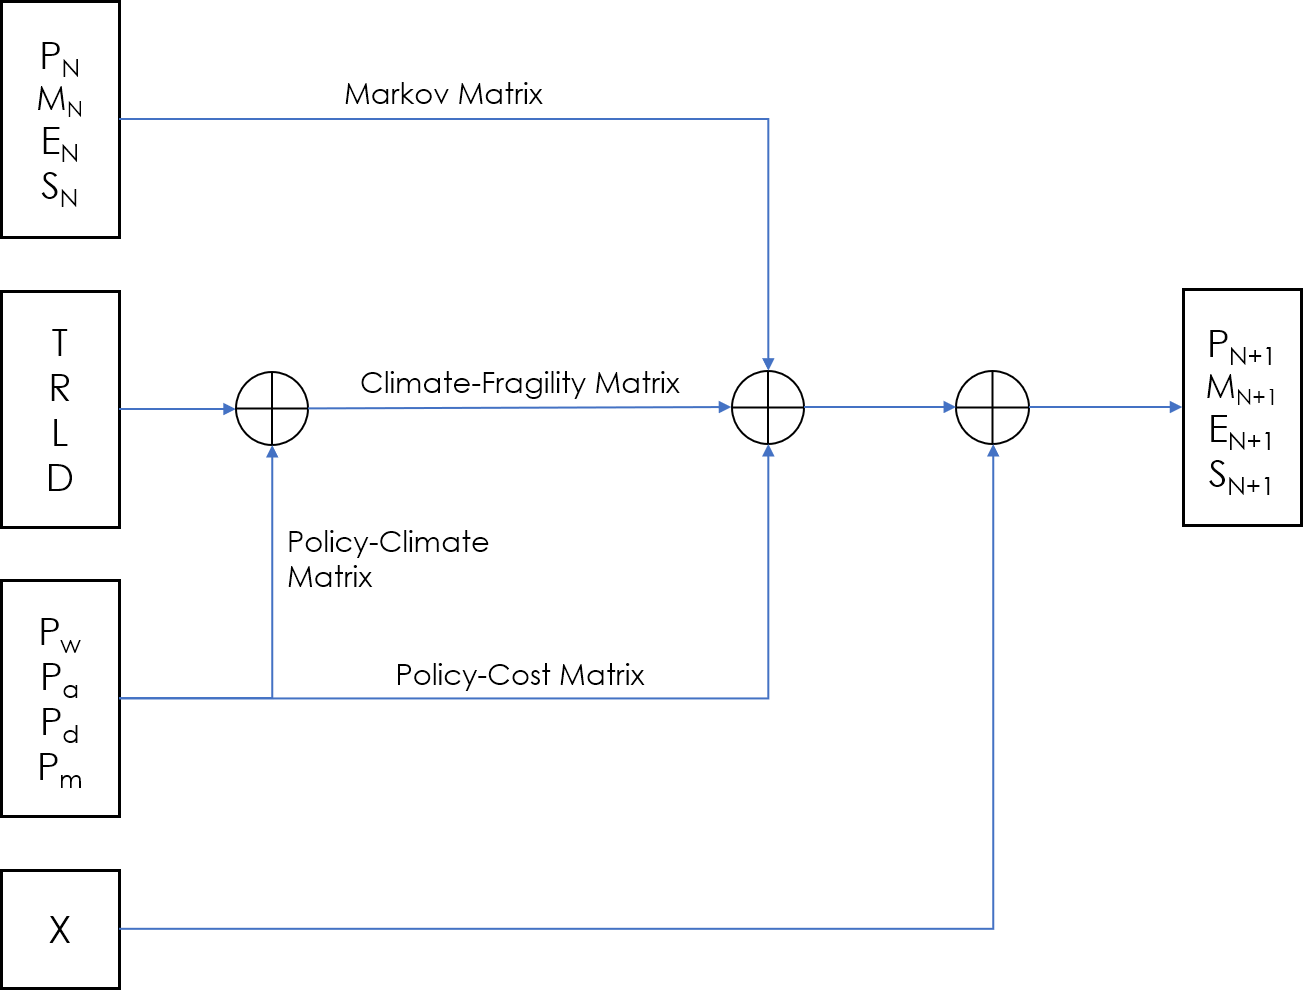
\includegraphics[width=14.5cm]{figure8.png}
\caption{$W_q-\lambda$ of different approaches} \label{fig:8}
\end{figure}
\section{Sensitivity analysis on cultural diversity}
Since passengers from different areas have their own customs and norms, their behaviors are different, which could possibly influence our model. In this chapter, we analyze three representative types of passengers and how their cultural diversities impact our model. In the end, we demonstrate how our model accommodate these differences. 
\subsection{Entrances paralyzed due to cutting in lines}
Passengers from some areas have the concept of prioritizing individual efficiency, so the probability of cutting in lines may increase. Meanwhile, if the dispute caused by cutting in lines can not be solved in time, it may lead to the temporary paralysis of an entrance.

We assume that the number of lanes paralyzed obeys Poisson Distribution. Due to scarcity of concrete data, we assume that it obeys $\pi(0.01)$. We have
$$P(S_{paralyzed}=k)=\frac{e^{-0.01}(0.01)^k}{k!}$$
From the calculation we can attain that the probability of a entrance paralyzed is approximately 1\%, of two entrances paralyzed is about 0.005\%, and of more entrances paralyzed is almost 0. Assumptions above are appropriate for the time period of general passenger flow. Therefore, we analyze the sensitivity according to the situation that there are only one or two entrances paralyzed.

Based on the previous optimization, we have already obtained that without the possibility of entrances paralyzed $W_q$ is about 20s, and no more than 40s .
\subsubsection{One entrance paralyzed}
From previous analysis, although the actual number of entrances is one less than the number we anticipate, it will result in the rapid increase of $W_q$. Assume that there is one entrance paralyzed, which means that passengers who are supposed to go through this entrance will wait in other entrances. The increase of other entrances should obey
$$\Delta L_q=\frac{\lambda\Delta t}{s(s-1)}$$
From what has been deduced before
$$s=\lceil\frac{\lambda}{\mu}-0.5\rceil+1$$
We have
$$\frac{dL_q}{dt}=\frac{\lambda}{\lceil\frac{\lambda}{\mu}-0.5\rceil(\lceil\frac{\lambda}{\mu}-0.5\rceil +1)}$$
\begin{figure}[h]
\small
\centering
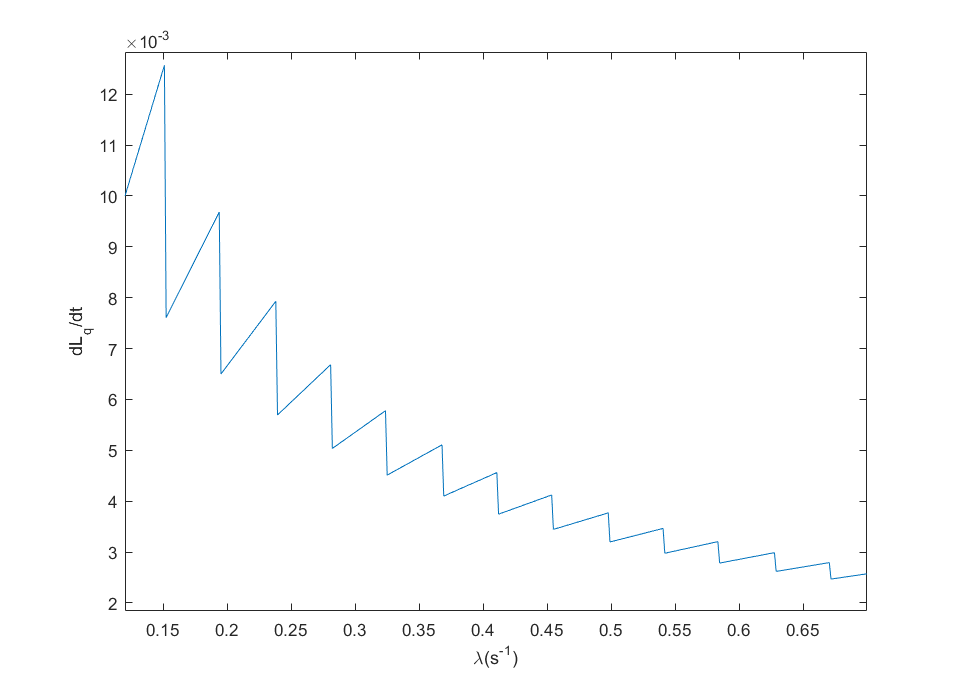
\includegraphics[width=10cm]{figure9.png}
\caption{$\frac{dL_q}{dt}-\lambda$ when one entrance paralyzed} \label{fig:9}
\end{figure}\\
Under such rule, when there is one entrance paralyzed, the speed of increases of the number of passengers waiting in other entrances is shown in \textbf{Figure 9}. We assume that most of disputes will be solved in five minutes. From the figure we can estimate that the number of people increasing for every entrance is 3.9, and is at most 4, which is to say, $W_q$ at most will increase by 1.5 minutes with the probability of 1\%.
\subsubsection{Two entrances paralyzed}
Similarly, when there are two entrances paralyzed, the speed of increases of the number of passengers for each entrances is
$$\frac{dL_q}{dt}=\frac{2\lambda}{\lceil\frac{\lambda}{\mu}-0.5\rceil(\lceil\frac{\lambda}{\mu}-0.5\rceil +1)}$$
If the flow of passengers is so little that the entrances open are less than two, the paralysis hardly happens. As a consequence, we omit the situation when $\lambda<0.1$ in the \textbf{Figure 10}.
\begin{figure}[h]
\small
\centering
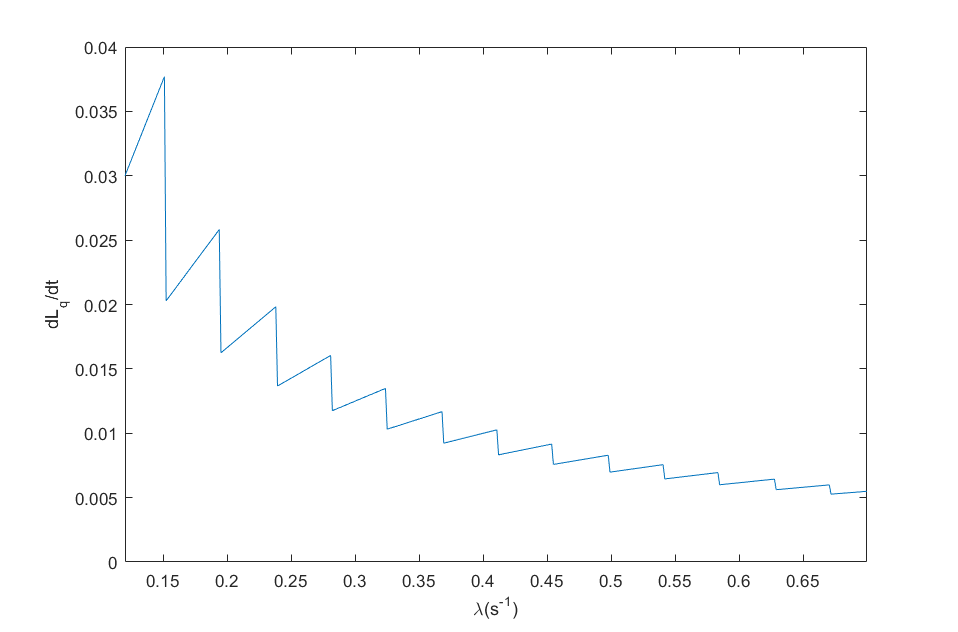
\includegraphics[width=10cm]{figure10.png}
\caption{$\frac{dL_q}{dt}-\lambda$ when two entrances paralyzed} \label{fig:10}
\end{figure}
Under such situation, we also assume that a dispute can be solved in five minutes. Thus, the increasing number of passengers for each entrance is at most 12. Passengers can markedly feel the increase of passengers, but the waiting time for each individual still will increase no more than 5 minutes.

The sensitivity analysis above is based on the distribution $\pi(0.01)$. If such paralyzing happens in a large scale, we do not need such model to analyze it. From our analysis, we can draw the conclusion that the influence of $W_q$ due to cutting in queues is small. To be more specific, the time will increase no more than 5 minutes.

\subsection{Longer screening time}
Passengers from different areas spend different time for security check. For instance, Egyptians and Jews are used to wearing kerchiefs while Americans are used to wearing simple jeans and T-shirt, which will absolutely result in different checking time.\\
Assume that in this case 
$$W_q'=1.2W_q$$ 
Then 
$$\mu'=\frac{1}{1.2}\mu=0.83\mu=0.0359$$ 
After calculation, the changed functional relationship is $s=\frac{\lambda }{0.0359}$. \textbf{Figure 11} shows $s-\lambda$, and \textbf{Figure 12} shows $W_q-\lambda$.
\begin{figure}[H]
\small
\centering
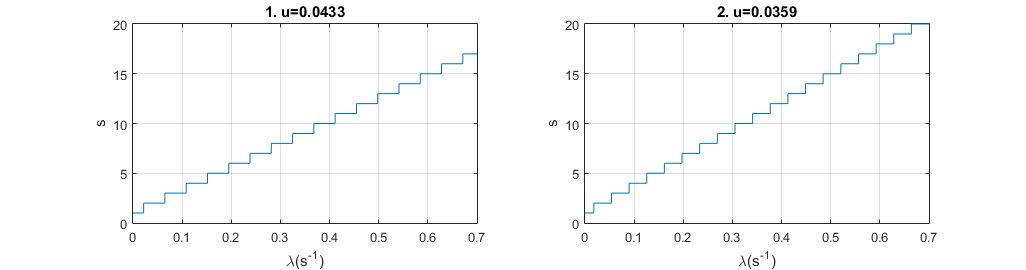
\includegraphics[width=15cm]{figure11.png}
\caption{$s-\lambda$ with longer screening time} \label{fig:11}
\end{figure}
\begin{figure}[h]
\small
\centering
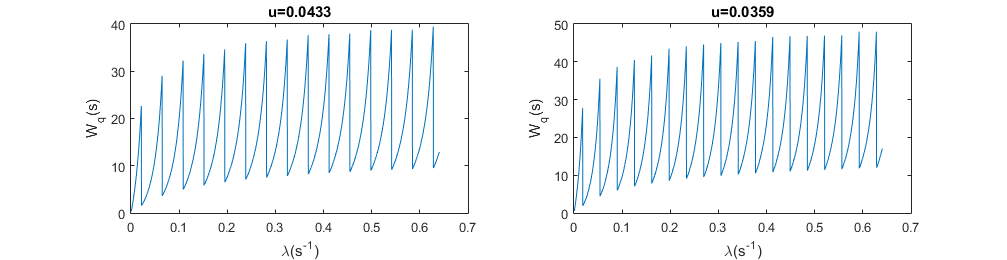
\includegraphics[width=15cm]{figure12.png}
\caption{$W_q-\lambda$ with longer screening time} \label{fig:12}
\end{figure}
 In this case, $\Delta W_q\leq \pm 24.0s$ when $W_q$ is constant (25s). Campared with the previous result $\Delta W_q\leq \pm 19.4s$, we can conclude that longer screening time due to different dressing has little impact on our model.

\subsection{More passengers getting additional screening}
Due to the culture discrepancies, passengers from different areas may have different understanding of definitions of contrabands. It is possible that some items are not allowed to take through the security checkpoint in some areas while such items can be safely carried in other areas. Furthermore, different countries have different norms of limited power of specific electronic equipments. Therefore, such discrepancies may lead to the increase of the probability of passengers from specific areas getting additional searching, which will decrease the efficiency of the whole system.

In the previous chapter, we assume that the proportion of passengers getting additional screening is a small constant $\eta$ whose influence on the whole system can be ignored. Now considering the influences of culture discrepancies, we assume that $\eta=0.02$ which is large enough to affect the throughput of passengers. Assume that the additional searching time also obey Exponential Distribution $E(\mu_D)$, and $\mu_D=\frac{1}{10}\mu_B$.
Then we have
$$\mu'=\frac{1}{\frac{\eta}{\mu_D}+\frac{1}{\mu_A}+\frac{1}{\mu_B}}=\frac{1}{\frac{10\eta}{\mu_B}+\frac{1}{\mu}}$$
Similarly, we show the relationship between $s-\lambda$ and $W_q-\lambda$ in \textbf{Figure 13} and \textbf{Figure 14}.
\begin{figure}[H]
\small
\centering
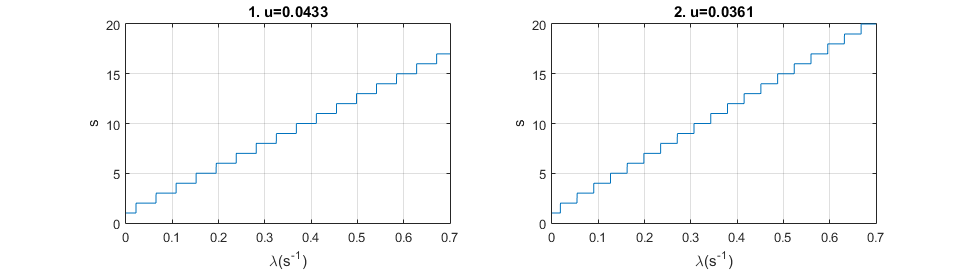
\includegraphics[width=15cm]{figure13.png}
\caption{$s-\lambda$ with more passengers in Zone D} \label{fig:13}
\end{figure}
\begin{figure}[H]
\small
\centering
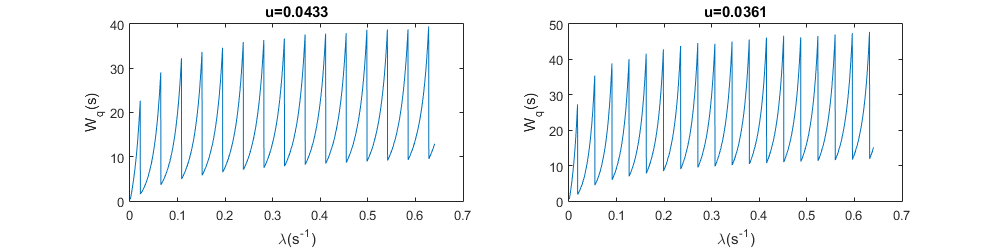
\includegraphics[width=15cm]{figure14.png}
\caption{$W_q-\lambda$ with more passengers in Zone D} \label{fig:14}
\end{figure}
When $W_q=25s$, we can calculate $\Delta W_q’\leq\pm23.9$. Campared with the previous result $\Delta W_q\leq \pm 19.4s$, we can safely draw theconclusion that more passengers in Zone D due to obsure perceptions of contraband have little impact on our model.
\section{Policy and recommendations}
\begin{itemize}
\item Based on the model established primitively, the speed of document check is twice over that of screening, as a consequence, the screening process contributes most to the appearance of bottlenecks. Therefore, the airport should dispatch more skilled TSA officers to the screening area and expedite the speed of screening.
\item Rationally arrange the number of entrances and lanes. From the optimization we have made, the best arrangement is shown below
$$N_X:N_B=2:1$$
$$\lambda_P:\lambda_R=3:2$$
$$N_X=1.2(N_P+N_R)$$
\item Monitor the flow of passengers in real time, and arrange the number of entrances according to the acquired values in order to reduce the cost on the basis of rational efficiency. The optimal result we obtain according to data we have is
$$s=\lceil\frac{\lambda}{\mu}-0.5\rceil+1$$
\item Arrange different number of TSA officers and security staffs in different security checkpoints in order to adjust the average waiting time of passengers. For instance, in the checkpoints with more queue-jumpers, we should arrange more staffs to insure that disputes caused by cutting will not continue for a long period. In the sensitivity analysis, the increasing velocity of queues satisfy that
$$\frac{dL_q}{dt}=\frac{\lambda s_{paralyzed}}{s(s-s_{paralyzed})}$$
We assumed that all kinds of disputes will be solved in five minutes, and if such time increases, the queue will be so long that passengers may suffer from anxiety.
\item Promote Pre-Check service, and increase the number of Pre-Check entrances, which will provide convenience to passengers and save the checking time. It is mentioned that 45\% of passengers enroll in Pre-Check, but since Pre-Check passengers tend to travel more frequently by plane, such proportion cannot be the criterion when deciding the number of Pre-Check entrances and regular entrances.
\item Establish a baggage buffer that used to temporarily store the baggage that has been checked. Since in our optimization each lane for body screening is accompanied with two lanes for baggage screening, which will increase the probability of baggage checked faster than passengers, such buffer can prevent the occurrence of congestion and improve the security level of baggage.
\item In the sensitivity analysis, we find that culture discrepancies will not impact greatly the queuing time, and the existing congestion mainly due to the insufficiency of entrances. Therefore, we propose that if cost permitting, the airport should open more entrances and disperse entrances as much as possible in order to disperse passengers, which will relief the anxiety of them.
\end{itemize}
\section{Strengths and weaknesses}
\subsection{Strengths}
\begin{itemize}
\item Our model separates the whole process of security check into ID-check part and screening part, and independently calculates the corresponding queuing conditions, which avoid the possible errors due to the complicated model.
\item We estimate the arrival rate for each passenger and the checking time for each TSA officer, and assume that the former obeys Poisson Distribution and the latter obeys Exponential Distribution, which conform to the general principles.
\item We apply the moment estimation to estimate relevant parameters of the system so as to obtain the basic model.
\item We apply the Queuing Theory, and consider the average waiting time and the flow of passengers as our principal evaluation indexes, which correspond with profits of airports and passengers.
\item When analyzing the sensitivity and improving the current model, we consider the difference of average waiting time and the maximal flow of passengers as our principal evaluation indexes, which guarantee that the airport can provide every passengers with the approximately same service with the maximal efficiency.
\end{itemize}
\subsection{Weaknesses}
\begin{itemize}
\item Since we do not have enough data, we have to estimate related parameters using moment estimation of data given. The error can be large when the data size is small.
\item The bound between service time and waiting time is not explicit enough. We assume that when passengers put their baggage on the belt, they finish waiting and service time begins, but actually perhaps passengers consider the time between the moment they put down their baggage and the moment they receive body screening is also the waiting time.\item Since we have less estimation of costs and utilization of space, our model considers efficiency and flying experience of passengers as the principal indexes. In fact, we should modify our model according to actual costs of airport construction.
\item We did not take the scale of the airport into account, and modeling based on the given data. If the scale of the airport is large enough, we need to rewrite some of our codes to obtain a more graceful result.
\end{itemize}

\begin{thebibliography}{99}
\bibitem{1}\url{https://en.wikipedia.org/wiki/Fragile_state#Defining_fragile_states}
\bibitem{2}Gan Y A, Tian F, Lee W Z, Lee M S, Chen B Z, Hu Y Q, Gu J F, Guo Y H, Qian S D. Operational research. Tsinghua University Press, 2005.
\bibitem{3}Clara V. Marin, Colin G. Drury, Rajan Batta, Li Lin. Server Adaptation in an Airport Security System Queue[J].The OR Society, 2007, Vol.20:22-31.
\bibitem{4}Zeng Junjie. Optimization and Configuration of Airport Security. Wide Angle, 2009:173-174.
\bibitem{5}MI Kamien,NL Schwartz. Dynamic Optimization: The Calculus of Variations and Optimal Control in Economics \& Management.North Holland, 1981, 31(1):1252-1257.
\bibitem{6}Zhang Guofen, Huang B Q, Zhang C Y. Probability Theory, Mathematical Statistics and Stochastic Process. Zhejiang University Press, 2011.
\bibitem{7}Ivo Adan, Jacques Resing. Queueing Systems.Department of Mathematics and Computing Science Eindhoven University of Technology, P.O. Box 513, 5600 MB Eindhoven, The Netherlands, 2015.
\bibitem{8}Queueing theory (https://en.wikipedia.org/wiki/Queueing\_theory).
\end{thebibliography}

\begin{appendices}

\section{First appendix}
Here are data  about how passengers proceed through each step of the security screening process. \\
\begin{table}[htbp]
\centering
\begin{tabular}{m{1.3cm}<{\centering}m{1.3cm}<{\centering}m{1.3cm}<{\centering}m{1.3cm}<{\centering}m{1.3cm}<{\centering}m{1.3cm}<{\centering}m{1.3cm}<{\centering}m{1.3cm}<{\centering}}
\toprule
\textbf{A}&\textbf{B}&\textbf{C}&\textbf{D}&\textbf{E}&\textbf{F}&\textbf{G}&\textbf{H}\\
\midrule					
00:00.&	00:00.&	00:08.&	00:15.&	00:09.&	00:03.&	00:00.&	0:48\\
00:11.&	00:09.&	00:05.&	00:12.&	00:20.&	00:06.&	00:02.&	0:45\\
00:13.&	00:10.&	00:11.&	00:15.&	00:33.&	00:07.&	00:03.&	0:28\\
00:14.&	00:11.&	00:10.&	00:20.&	00:36.&	00:09.&	00:11.&	0:25\\
00:15.&	00:13.&	00:09.&	00:08.&	00:43.&	00:20.&		&	0:22\\
00:25.&	00:14.&	00:09.&	00:08.&	00:52.&	00:22.&		&	0:24\\
00:34.&	00:16.&	00:13.&	00:11.&	01:05.&	00:25.&		&	0:17\\
00:54.&	00:27.&	00:15.&		&	01:16.&	00:41.&		&	0:33\\
00:56.&	00:57.&	00:12.&		&	01:25.&	01:07.&		&	0:08\\
01:15.&	01:21.&		&		&	01:32.&	01:09.&		&	0:10\\
01:16.&	02:16.&		&		&	01:43.&	01:18.&		&	0:26\\
01:44.&	02:24.&		&		&	01:58.&		&		&	0:32\\
01:49.&	02:27.&		&		&	02:09.&		&		&	0:21\\
02:04.&	02:43.&		&		&	02:26.&		&		&	0:37\\
02:26.&	02:44.&		&		&	02:40.&		&		&	1:08\\
					
\bottomrule
\end{tabular}
\end{table}
\begin{table}[htbp]
\centering
\begin{tabular}{m{1.3cm}<{\centering}m{1.3cm}<{\centering}m{1.3cm}<{\centering}m{1.3cm}<{\centering}m{1.3cm}<{\centering}m{1.3cm}<{\centering}m{1.3cm}<{\centering}m{1.3cm}<{\centering}}
\toprule
\textbf{A}&\textbf{B}&\textbf{C}&\textbf{D}&\textbf{E}&\textbf{F}&\textbf{G}&\textbf{H}\\
\midrule
02:54.&	03:06.&		&		&	02:47.&		&		&	0:40\\
02:58.&	03:13.&		&		&	02:54.&		&		&	0:18\\
02:59.&	03:15.&		&		&	03:06.&		&		&	0:26\\
03:01.&	03:27.&		&		&	03:25.&		&		&	0:08\\
03:06.&	03:29.&		&		&	03:34.&		&		&	0:21\\
03:09.&	04:27.&		&		&	04:11.&		&		&	0:23\\
03:10.&	04:42.&		&		&	04:22.&		&		&	0:28\\
03:20.&	04:48.&		&		&	04:35.&		&		&	0:50\\
03:22.&	05:00.&		&		&	04:47.&		&		&	0:28\\
03:34.&	05:09.&		&		&	05:00.&		&		&	0:48\\
03:53.&	05:40.&		&		&	05:11.&		&		&	0:28\\
04:17.&	05:57.&		&		&	05:18.&		&		&	0:36\\
04:35.&	06:00.&		&		&	05:26.&		&		&	0:27\\
04:36.&	06:20.&		&		&	05:41.&		&		&	0:05\\
04:37.&	07:39.&		&		&	05:48.&&&\\		
04:38.&	07:51.&		&		&	05:59.&&&\\			
05:06.&	08:01.&		&		&	06:09.&&&\\			
05:13.&	08:02.&		&		&	06:36.&&&\\			
05:37.&	08:04.&		&		&	06:45.&&&\\			
05:42.&	08:06.&		&		&	06:54.&&&\\		
05:46.&	08:18.&		&		&	07:05.&&&\\			
06:03.&	08:20.&		&		&	07:15.&&&\\			
06:06.&	08:21.&		&		&	07:24.&&&\\			
06:11.&	08:22.&		&		&	07:36.&&&\\			
06:46.&	08:33.&		&		&	07:43.&&&\\		
06:47.&	08:46.&&&&&&\\						
06:49.&	08:54.&&&&&&\\						
06:50.&	08:56.&&&&&&\\						
07:06.&	09:13.&&&&&&\\						
07:07.&	09:34.&&&&&&\\						
07:27.&	09:53.&&&&&&\\						
07:36.&	09:56.&&&&&&\\	
07:41.&&&&&&&\\							
07:41.&&&&&&&\\						
07:42.&&&&&&&\\							
07:47.&&&&&&&\\							
08:16.&&&&&&&\\							
08:23.&&&&&&&\\							
08:25.&&&&&&&\\							
08:26.&&&&&&&\\							
08:27.&&&&&&&\\							
08:43.&&&&&&&\\							
08:44.&&&&&&&\\							
\bottomrule
\end{tabular}
\end{table}

\begin{table}[htbp]
\centering
\begin{tabular}{m{1.2cm}<{\centering}|m{3cm}<{\centering}|m{9cm}<{\centering}}
\whline
\textbf{Symbol}&\textbf{Process}&\textbf{Notes}\\
\hline 
A&TSA PreCheck Arrival Times&	Airport checkpoint recoding individuals entering the pre-check queue.\\
\hline 
B&Regular Arrival Times	&Airport checkpoint recoding individuals entering the regular queue.\\
\hline 
C&ID Check TSA officer 1	&The time the arrival of the passenger to the ID check station until the TSA officer calls the next passenger forward.\\
\hline 
D&ID Check TSA officer 2	&Same as column C, but for a different TSA officer.\\
\hline 
E&mm wave scan times	&Time stamps as passenger exited the milimeter wave scanner.\\
\hline 
F&X-Ray Scan Time 1	&Time stamps as bags exited the x-ray screening.\\
\hline 
G&X-Ray Scan Time 2	&Same as column F, but for a different TSA officer.\\
\hline  
H&Time to get scanned property	&Time it takes people from arriving at the belt to place items to be scanned, until they retrieved their items off the post-xray belt.\\
\shline
\end{tabular}
\end{table}







  

\section{Second appendix}
Here are simulation programmes we used in our model as follow.

\noindent \textbf{\textcolor[rgb]{0.98,0.00,0.00}{Draw the figure of $f_{omax}$ and $N_L/N_P$}}
\lstinputlisting[language=Matlab]{./code/fomax_NL_NP.m}
\textbf{\textcolor[rgb]{0.98,0.00,0.00}{Find the zero point of the function $test$ }}
\lstinputlisting[language=Matlab]{./code/drive_test.m}
\textbf{\textcolor[rgb]{0.98,0.00,0.00}{Calculate $W_q$ for every specific $s$}}
\lstinputlisting[language=Matlab]{./code/test.m}
\textbf{\textcolor[rgb]{0.98,0.00,0.00}{Draw figures of $s$ and $\lambda$ when approaches to rounding $s$ are different}}
\lstinputlisting[language=Matlab]{./code/s_lambda1.m}
\textbf{\textcolor[rgb]{0.98,0.00,0.00}{Draw figures of $W_q$ and $\lambda$ when approaches to rounding $s$ are different}}
\lstinputlisting[language=Matlab]{./code/Wq_lambda1.m}
\textbf{\textcolor[rgb]{0.98,0.00,0.00}{Draw figures of $s$ and $\lambda$ when screening time is longer}}
\lstinputlisting[language=Matlab]{./code/s_lambda2.m}
\textbf{\textcolor[rgb]{0.98,0.00,0.00}{Draw figures of $W_q$ and $\lambda$ when screening time is longer}}
\lstinputlisting[language=Matlab]{./code/Wq_lambda2.m}
\textbf{\textcolor[rgb]{0.98,0.00,0.00}{Draw figures of $s$ and $\lambda$ when there are more passengers entering Zone D}}
\lstinputlisting[language=Matlab]{./code/s_lambda3.m}
\textbf{\textcolor[rgb]{0.98,0.00,0.00}{Draw figures of $W_q$ and $\lambda$ when there are more passengers entering Zone D}}
\lstinputlisting[language=Matlab]{./code/Wq_lambda3.m}
\noindent \textbf{\textcolor[rgb]{0.98,0.00,0.00}{Draw the figure of $dW_q/dt-\lambda$ when there is one entrance paralyzed}}
\lstinputlisting[language=Matlab]{./code/OneEntranceParalyzed.m}
\textbf{\textcolor[rgb]{0.98,0.00,0.00}{Draw the figure of $dW_q/dt-\lambda$ when there are two entrances paralyzed }}
\lstinputlisting[language=Matlab]{./code/TwoEntranceParalyzed.m}
\end{appendices}
\end{document}

%% 
%% This work consists of these files mcmthesis.dtx,
%%                                   figures/ and
%%                                   code/,
%% and the derived files             mcmthesis.cls,
%%                                   mcmthesis-demo.tex,
%%                                   README,
%%                                   LICENSE,
%%                                   mcmthesis.pdf and
%%                                   mcmthesis-demo.pdf.
%%
%% End of file `mcmthesis-demo.tex'.
